\documentclass[tikz,crop,convert={density=200,outext=.png},border=0.4cm]{standalone}

\usepackage{pgfplots}
\usepackage{amsmath}
\usetikzlibrary{arrows.meta}
\usepackage{physics}
\usepackage{xcolor}
\definecolor{mixed_1}{RGB}{2,56,88}
\definecolor{mixed_2}{RGB}{54,144,192}
\definecolor{mixed_3}{RGB}{208,209,230}
\definecolor{pow_1}{RGB}{103,0,31}
\definecolor{pow_2}{RGB}{206,18,86}
\definecolor{pow_3}{RGB}{223,101,176}
\pgfplotsset{compat=newest,
    %width=6cm,
    %height=3cm,
    scale only axis=true,
    max space between ticks=25pt,
    try min ticks=5,
    every axis/.style={
        axis y line=middle,
        axis x line=middle,
        axis line style={thick,->,>=latex, shorten >=-.3cm}
    },
    every axis plot/.append style={thick},
    tick style={black, thick},
}
\tikzset{
    semithick/.style={line width=0.8pt},
}
\usepgfplotslibrary{groupplots}
\usepgfplotslibrary{dateplot}
% Document begins
\begin{document}
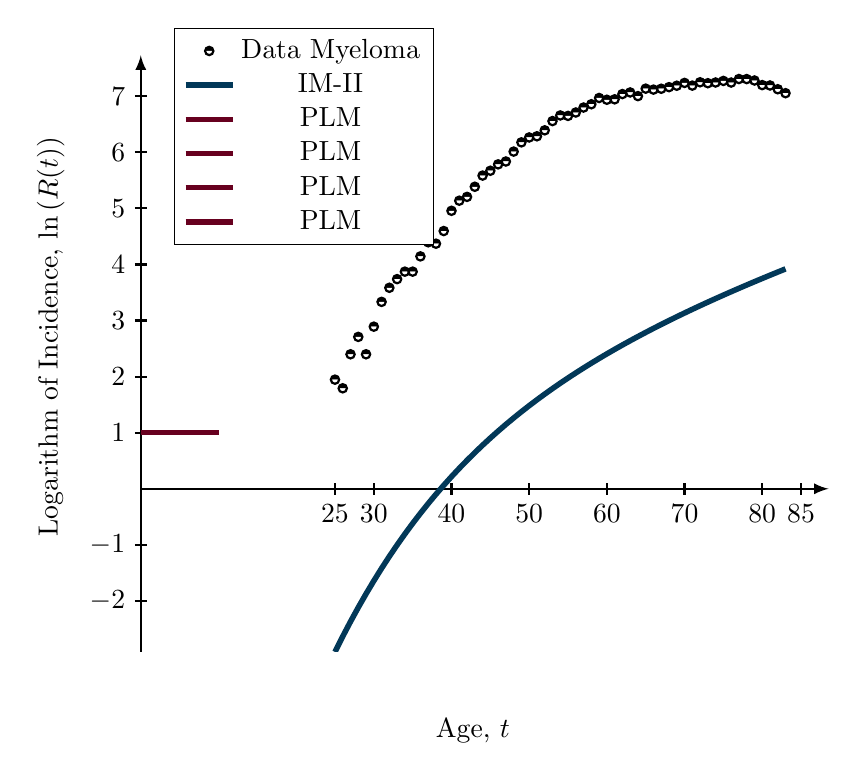
\begin{tikzpicture}
  % The axis of the plot
\begin{axis}[
    %title={Model: $\dv{y}{t}=\frac{2y}{t}$ with solution $y(t)=C_1t^2$\\Symmetry: $\Gamma_{\epsilon}=(t,y)\mapsto\left(\exp\left(\epsilon\right)t,\exp\left(-\epsilon\right)y\right)$},
    title style = {align=left},
    xlabel={Age, $t$},
    %ylabel={Incidence, $R(t)$},
    ylabel={Logarithm of Incidence, $\ln\left(R(t)\right)$},    
    % ylabel={Incidence, $R(t)$},
    x label style={at={(axis description cs:0.5,-0.1)},anchor=north},
    y label style={at={(axis description cs:-0.1,0.55)},rotate=90,anchor=south},    
    % xmin=-27, xmax=5,
    xmin=0, xmax=85.5,
    %ymin=-20, ymax=20,
    xtick={0,25,30,40,...,80,85},
    %ymin=-20, ymax=20,
    %xtick={-30,-27,...,9},
    %ytick={-15,-10,...,15},
    legend style={at={(axis description cs:0.05,0.9)},anchor=west},    
    %legend pos=north west,
    %ymajorgrids=true,
    grid style=dashed,
]
% Plot the data
\addplot[
only marks, mark=halfcircle*,mark size=1.5pt,color=black,
]
coordinates {%
(25.0,1.9459101490553132)
(26.0,1.791759469228055)
(27.0,2.3978952727983707)
(28.0,2.70805020110221)
(29.0,2.3978952727983707)
(30.0,2.8903717578961645)
(31.0,3.332204510175204)
(32.0,3.58351893845611)
(33.0,3.7376696182833684)
(34.0,3.871201010907891)
(35.0,3.871201010907891)
(36.0,4.143134726391533)
(37.0,4.394449154672439)
(38.0,4.3694478524670215)
(39.0,4.59511985013459)
(40.0,4.955827057601261)
(41.0,5.135798437050262)
(42.0,5.204006687076795)
(43.0,5.384495062789089)
(44.0,5.583496308781699)
(45.0,5.66988092298052)
(46.0,5.783825182329737)
(47.0,5.834810737062605)
(48.0,6.0112671744041615)
(49.0,6.175867270105761)
(50.0,6.263398262591624)
(51.0,6.284134161070802)
(52.0,6.39024066706535)
(53.0,6.555356891810665)
(54.0,6.655440350367647)
(55.0,6.647688373563329)
(56.0,6.70808408385307)
(57.0,6.796823718274855)
(58.0,6.855408798609928)
(59.0,6.966967138613983)
(60.0,6.93537044601511)
(61.0,6.943122422819428)
(62.0,7.037027614686276)
(63.0,7.065613363597717)
(64.0,7.00033446027523)
(65.0,7.133295954896068)
(66.0,7.116394144093465)
(67.0,7.1316985104669115)
(68.0,7.160069207596127)
(69.0,7.1853870155804165)
(70.0,7.23561914106675)
(71.0,7.187657164114956)
(72.0,7.247080584585756)
(73.0,7.2305631534092925)
(74.0,7.242797922793756)
(75.0,7.271008538280992)
(76.0,7.242082359256962)
(77.0,7.305188215393037)
(78.0,7.303843225277705)
(79.0,7.278628942320682)
(80.0,7.19668657083435)
(81.0,7.189922170745808)
(82.0,7.122866658599083)
(83.0,7.052721049232323)
};
\addlegendentry{Data Myeloma}

% Plot the IM-II model
\addplot[
color=mixed_1,line width=2pt,
]
coordinates {%
(25.0,-2.907084451511482)
(26.0,-2.631447322340589)
(27.0,-2.367517805325354)
(28.0,-2.1147615791913164)
(29.0,-1.8726639178560034)
(30.0,-1.6407288990903441)
(31.0,-1.418478712867064)
(32.0,-1.205453062331872)
(33.0,-1.0012086481711253)
(34.0,-0.8053187254591445)
(35.0,-0.617372720933973)
(36.0,-0.4369758981081917)
(37.0,-0.26374905765936907)
(38.0,-0.09732826111052217)
(39.0,0.0626354331791723)
(40.0,0.216476231343123)
(41.0,0.36451387070743513)
(42.0,0.507053898219934)
(43.0,0.6443879652561422)
(44.0,0.7767941418115405)
(45.0,0.904537251588724)
(46.0,1.0278692281724489)
(47.0,1.1470294913832588)
(48.0,1.2622453420223114)
(49.0,1.373732372563233)
(50.0,1.4816948908973613)
(51.0,1.5863263539752464)
(52.0,1.687809808083842)
(53.0,1.7863183325274714)
(54.0,1.8820154836136225)
(55.0,1.9750557360555399)
(56.0,2.065584919168738)
(57.0,2.1537406455373174)
(58.0,2.2396527301410663)
(59.0,2.3234435982519295)
(60.0,2.4052286807176904)
(61.0,2.485116795543802)
(62.0,2.5632105149556894)
(63.0,2.639606517370164)
(64.0,2.7143959239240436)
(65.0,2.7876646194002666)
(66.0,2.859493557557238)
(67.0,2.929959051007113)
(68.0,2.99913304590495)
(69.0,3.0670833818051815)
(70.0,3.1338740371168163)
(71.0,3.1995653606464773)
(72.0,3.264214289760856)
(73.0,3.3278745557296543)
(74.0,3.390596876828349)
(75.0,3.45242913978907)
(76.0,3.513416570189003)
(77.0,3.573601892360515)
(78.0,3.6330254793968724)
(79.0,3.6917254938130397)
(80.0,3.7497380194035936)
(81.0,3.807097184820018)
(82.0,3.8638352793682778)
(83.0,3.9199828615050936)
};
\addlegendentry{IM-II}

% Plot the PLM model
\addplot[
color=pow_1,line width=2pt,
]
coordinates {%
(0.0,1.0)
(0.10101010101010101,1.000000000000051)
(0.20202020202020202,0.999999999998303)
(0.30303030303030304,1.0000000000001539)
(0.40404040404040403,0.9999999999983028)
(0.5050505050505051,1.0000000000002565)
(0.6060606060606061,1.000000000000307)
(0.7070707070707071,0.999999999998303)
(0.8080808080808081,1.0000000000004097)
(0.9090909090909091,1.0000000000004612)
(1.0101010101010102,0.9999999999983027)
(1.1111111111111112,1.0000000000005638)
(1.2121212121212122,0.9999999999983029)
(1.3131313131313131,0.9999999999983028)
(1.4141414141414141,0.9999999999983028)
(1.5151515151515151,1.0000000000007685)
(1.6161616161616161,0.9999999999983029)
(1.7171717171717171,1.000000000000871)
(1.8181818181818181,0.9999999999983028)
(1.9191919191919191,1.0000000000009743)
(2.0202020202020203,1.0000000000010254)
(2.121212121212121,1.0000000000010765)
(2.2222222222222223,1.000000000001128)
(2.323232323232323,1.0000000000011795)
(2.4242424242424243,0.9999999999983029)
(2.525252525252525,0.9999999999983028)
(2.6262626262626263,1.0000000000013323)
(2.727272727272727,0.9999999999983029)
(2.8282828282828283,0.9999999999983028)
(2.929292929292929,0.9999999999983029)
(3.0303030303030303,0.9999999999983029)
(3.131313131313131,1.0000000000015896)
(3.2323232323232323,0.9999999999983029)
(3.3333333333333335,0.9999999999983028)
(3.4343434343434343,0.999999999998303)
(3.5353535353535355,1.0000000000017943)
(3.6363636363636362,1.0000000000018454)
(3.7373737373737375,1.0000000000018974)
(3.8383838383838382,1.0000000000019478)
(3.9393939393939394,1.0000000000019993)
(4.040404040404041,1.0000000000020506)
(4.141414141414141,0.9999999999983028)
(4.242424242424242,0.9999999999983029)
(4.343434343434343,0.9999999999983028)
(4.444444444444445,1.0000000000022569)
(4.545454545454545,1.0000000000023075)
(4.646464646464646,0.9999999999983028)
(4.747474747474747,0.9999999999983029)
(4.848484848484849,1.0000000000024623)
(4.94949494949495,1.000000000002512)
(5.05050505050505,0.999999999998303)
(5.151515151515151,1.0000000000026144)
(5.252525252525253,1.0000000000026665)
(5.353535353535354,1.000000000002718)
(5.454545454545454,0.9999999999983027)
(5.555555555555555,1.0000000000028204)
(5.656565656565657,1.0000000000028708)
(5.757575757575758,1.0000000000029228)
(5.858585858585858,0.9999999999983029)
(5.959595959595959,0.9999999999983027)
(6.0606060606060606,1.0000000000030764)
(6.161616161616162,1.0000000000031275)
(6.262626262626262,1.0000000000031783)
(6.363636363636363,1.0000000000032296)
(6.4646464646464645,1.000000000003282)
(6.565656565656566,1.0000000000033318)
(6.666666666666667,1.000000000003384)
(6.767676767676767,1.0000000000034348)
(6.8686868686868685,1.0000000000034859)
(6.96969696969697,0.9999999999983027)
(7.070707070707071,1.00000000000359)
(7.171717171717171,1.000000000003641)
(7.2727272727272725,1.0000000000036908)
(7.373737373737374,0.999999999998303)
(7.474747474747475,1.000000000003795)
(7.575757575757575,0.9999999999983027)
(7.6767676767676765,1.0000000000038956)
(7.777777777777778,0.9999999999983027)
(7.878787878787879,0.9999999999983029)
(7.979797979797979,1.0000000000040505)
(8.080808080808081,1.0000000000041016)
(8.181818181818182,1.0000000000041547)
(8.282828282828282,0.9999999999983031)
(8.383838383838384,0.9999999999983029)
(8.484848484848484,1.0000000000043072)
(8.585858585858587,1.0000000000043585)
(8.686868686868687,0.999999999998303)
(8.787878787878787,1.0000000000044604)
(8.88888888888889,0.9999999999983029)
(8.98989898989899,1.0000000000045648)
(9.09090909090909,1.000000000004614)
(9.191919191919192,1.0000000000046658)
(9.292929292929292,1.000000000004718)
(9.393939393939394,1.000000000004769)
(9.494949494949495,0.9999999999983032)
(9.595959595959595,1.0000000000048725)
(9.696969696969697,1.0000000000049225)
(9.797979797979798,1.0000000000049725)
(9.8989898989899,1.0000000000050229)
(10.0,1.0000000000050784)
};
\addlegendentry{PLM}
\addplot[
color=pow_1,line width=2pt,
]
coordinates {%
(0.0,1.0)
(0.10101010101010101,1.000000000000051)
(0.20202020202020202,0.999999999998303)
(0.30303030303030304,1.0000000000001539)
(0.40404040404040403,0.9999999999983028)
(0.5050505050505051,1.0000000000002565)
(0.6060606060606061,1.000000000000307)
(0.7070707070707071,0.999999999998303)
(0.8080808080808081,1.0000000000004097)
(0.9090909090909091,1.0000000000004612)
(1.0101010101010102,0.9999999999983027)
(1.1111111111111112,1.0000000000005638)
(1.2121212121212122,0.9999999999983029)
(1.3131313131313131,0.9999999999983028)
(1.4141414141414141,0.9999999999983028)
(1.5151515151515151,1.0000000000007685)
(1.6161616161616161,0.9999999999983029)
(1.7171717171717171,1.000000000000871)
(1.8181818181818181,0.9999999999983028)
(1.9191919191919191,1.0000000000009743)
(2.0202020202020203,1.0000000000010254)
(2.121212121212121,1.0000000000010765)
(2.2222222222222223,1.000000000001128)
(2.323232323232323,1.0000000000011795)
(2.4242424242424243,0.9999999999983029)
(2.525252525252525,0.9999999999983028)
(2.6262626262626263,1.0000000000013323)
(2.727272727272727,0.9999999999983029)
(2.8282828282828283,0.9999999999983028)
(2.929292929292929,0.9999999999983029)
(3.0303030303030303,0.9999999999983029)
(3.131313131313131,1.0000000000015896)
(3.2323232323232323,0.9999999999983029)
(3.3333333333333335,0.9999999999983028)
(3.4343434343434343,0.999999999998303)
(3.5353535353535355,1.0000000000017943)
(3.6363636363636362,1.0000000000018454)
(3.7373737373737375,1.0000000000018974)
(3.8383838383838382,1.0000000000019478)
(3.9393939393939394,1.0000000000019993)
(4.040404040404041,1.0000000000020506)
(4.141414141414141,0.9999999999983028)
(4.242424242424242,0.9999999999983029)
(4.343434343434343,0.9999999999983028)
(4.444444444444445,1.0000000000022569)
(4.545454545454545,1.0000000000023075)
(4.646464646464646,0.9999999999983028)
(4.747474747474747,0.9999999999983029)
(4.848484848484849,1.0000000000024623)
(4.94949494949495,1.000000000002512)
(5.05050505050505,0.999999999998303)
(5.151515151515151,1.0000000000026144)
(5.252525252525253,1.0000000000026665)
(5.353535353535354,1.000000000002718)
(5.454545454545454,0.9999999999983027)
(5.555555555555555,1.0000000000028204)
(5.656565656565657,1.0000000000028708)
(5.757575757575758,1.0000000000029228)
(5.858585858585858,0.9999999999983029)
(5.959595959595959,0.9999999999983027)
(6.0606060606060606,1.0000000000030764)
(6.161616161616162,1.0000000000031275)
(6.262626262626262,1.0000000000031783)
(6.363636363636363,1.0000000000032296)
(6.4646464646464645,1.000000000003282)
(6.565656565656566,1.0000000000033318)
(6.666666666666667,1.000000000003384)
(6.767676767676767,1.0000000000034348)
(6.8686868686868685,1.0000000000034859)
(6.96969696969697,0.9999999999983027)
(7.070707070707071,1.00000000000359)
(7.171717171717171,1.000000000003641)
(7.2727272727272725,1.0000000000036908)
(7.373737373737374,0.999999999998303)
(7.474747474747475,1.000000000003795)
(7.575757575757575,0.9999999999983027)
(7.6767676767676765,1.0000000000038956)
(7.777777777777778,0.9999999999983027)
(7.878787878787879,0.9999999999983029)
(7.979797979797979,1.0000000000040505)
(8.080808080808081,1.0000000000041016)
(8.181818181818182,1.0000000000041547)
(8.282828282828282,0.9999999999983031)
(8.383838383838384,0.9999999999983029)
(8.484848484848484,1.0000000000043072)
(8.585858585858587,1.0000000000043585)
(8.686868686868687,0.999999999998303)
(8.787878787878787,1.0000000000044604)
(8.88888888888889,0.9999999999983029)
(8.98989898989899,1.0000000000045648)
(9.09090909090909,1.000000000004614)
(9.191919191919192,1.0000000000046658)
(9.292929292929292,1.000000000004718)
(9.393939393939394,1.000000000004769)
(9.494949494949495,0.9999999999983032)
(9.595959595959595,1.0000000000048725)
(9.696969696969697,1.0000000000049225)
(9.797979797979798,1.0000000000049725)
(9.8989898989899,1.0000000000050229)
(10.0,1.0000000000050784)
};
\addlegendentry{PLM}
\addplot[
color=pow_1,line width=2pt,
]
coordinates {%
(0.0,1.0)
(0.10101010101010101,1.000000000000051)
(0.20202020202020202,0.999999999998303)
(0.30303030303030304,1.0000000000001539)
(0.40404040404040403,0.9999999999983028)
(0.5050505050505051,1.0000000000002565)
(0.6060606060606061,1.000000000000307)
(0.7070707070707071,0.999999999998303)
(0.8080808080808081,1.0000000000004097)
(0.9090909090909091,1.0000000000004612)
(1.0101010101010102,0.9999999999983027)
(1.1111111111111112,1.0000000000005638)
(1.2121212121212122,0.9999999999983029)
(1.3131313131313131,0.9999999999983028)
(1.4141414141414141,0.9999999999983028)
(1.5151515151515151,1.0000000000007685)
(1.6161616161616161,0.9999999999983029)
(1.7171717171717171,1.000000000000871)
(1.8181818181818181,0.9999999999983028)
(1.9191919191919191,1.0000000000009743)
(2.0202020202020203,1.0000000000010254)
(2.121212121212121,1.0000000000010765)
(2.2222222222222223,1.000000000001128)
(2.323232323232323,1.0000000000011795)
(2.4242424242424243,0.9999999999983029)
(2.525252525252525,0.9999999999983028)
(2.6262626262626263,1.0000000000013323)
(2.727272727272727,0.9999999999983029)
(2.8282828282828283,0.9999999999983028)
(2.929292929292929,0.9999999999983029)
(3.0303030303030303,0.9999999999983029)
(3.131313131313131,1.0000000000015896)
(3.2323232323232323,0.9999999999983029)
(3.3333333333333335,0.9999999999983028)
(3.4343434343434343,0.999999999998303)
(3.5353535353535355,1.0000000000017943)
(3.6363636363636362,1.0000000000018454)
(3.7373737373737375,1.0000000000018974)
(3.8383838383838382,1.0000000000019478)
(3.9393939393939394,1.0000000000019993)
(4.040404040404041,1.0000000000020506)
(4.141414141414141,0.9999999999983028)
(4.242424242424242,0.9999999999983029)
(4.343434343434343,0.9999999999983028)
(4.444444444444445,1.0000000000022569)
(4.545454545454545,1.0000000000023075)
(4.646464646464646,0.9999999999983028)
(4.747474747474747,0.9999999999983029)
(4.848484848484849,1.0000000000024623)
(4.94949494949495,1.000000000002512)
(5.05050505050505,0.999999999998303)
(5.151515151515151,1.0000000000026144)
(5.252525252525253,1.0000000000026665)
(5.353535353535354,1.000000000002718)
(5.454545454545454,0.9999999999983027)
(5.555555555555555,1.0000000000028204)
(5.656565656565657,1.0000000000028708)
(5.757575757575758,1.0000000000029228)
(5.858585858585858,0.9999999999983029)
(5.959595959595959,0.9999999999983027)
(6.0606060606060606,1.0000000000030764)
(6.161616161616162,1.0000000000031275)
(6.262626262626262,1.0000000000031783)
(6.363636363636363,1.0000000000032296)
(6.4646464646464645,1.000000000003282)
(6.565656565656566,1.0000000000033318)
(6.666666666666667,1.000000000003384)
(6.767676767676767,1.0000000000034348)
(6.8686868686868685,1.0000000000034859)
(6.96969696969697,0.9999999999983027)
(7.070707070707071,1.00000000000359)
(7.171717171717171,1.000000000003641)
(7.2727272727272725,1.0000000000036908)
(7.373737373737374,0.999999999998303)
(7.474747474747475,1.000000000003795)
(7.575757575757575,0.9999999999983027)
(7.6767676767676765,1.0000000000038956)
(7.777777777777778,0.9999999999983027)
(7.878787878787879,0.9999999999983029)
(7.979797979797979,1.0000000000040505)
(8.080808080808081,1.0000000000041016)
(8.181818181818182,1.0000000000041547)
(8.282828282828282,0.9999999999983031)
(8.383838383838384,0.9999999999983029)
(8.484848484848484,1.0000000000043072)
(8.585858585858587,1.0000000000043585)
(8.686868686868687,0.999999999998303)
(8.787878787878787,1.0000000000044604)
(8.88888888888889,0.9999999999983029)
(8.98989898989899,1.0000000000045648)
(9.09090909090909,1.000000000004614)
(9.191919191919192,1.0000000000046658)
(9.292929292929292,1.000000000004718)
(9.393939393939394,1.000000000004769)
(9.494949494949495,0.9999999999983032)
(9.595959595959595,1.0000000000048725)
(9.696969696969697,1.0000000000049225)
(9.797979797979798,1.0000000000049725)
(9.8989898989899,1.0000000000050229)
(10.0,1.0000000000050784)
};
\addlegendentry{PLM}
\addplot[
color=pow_1,line width=2pt,
]
coordinates {%
(0.0,1.0)
(0.10101010101010101,1.000000000000051)
(0.20202020202020202,0.999999999998303)
(0.30303030303030304,1.0000000000001539)
(0.40404040404040403,0.9999999999983028)
(0.5050505050505051,1.0000000000002565)
(0.6060606060606061,1.000000000000307)
(0.7070707070707071,0.999999999998303)
(0.8080808080808081,1.0000000000004097)
(0.9090909090909091,1.0000000000004612)
(1.0101010101010102,0.9999999999983027)
(1.1111111111111112,1.0000000000005638)
(1.2121212121212122,0.9999999999983029)
(1.3131313131313131,0.9999999999983028)
(1.4141414141414141,0.9999999999983028)
(1.5151515151515151,1.0000000000007685)
(1.6161616161616161,0.9999999999983029)
(1.7171717171717171,1.000000000000871)
(1.8181818181818181,0.9999999999983028)
(1.9191919191919191,1.0000000000009743)
(2.0202020202020203,1.0000000000010254)
(2.121212121212121,1.0000000000010765)
(2.2222222222222223,1.000000000001128)
(2.323232323232323,1.0000000000011795)
(2.4242424242424243,0.9999999999983029)
(2.525252525252525,0.9999999999983028)
(2.6262626262626263,1.0000000000013323)
(2.727272727272727,0.9999999999983029)
(2.8282828282828283,0.9999999999983028)
(2.929292929292929,0.9999999999983029)
(3.0303030303030303,0.9999999999983029)
(3.131313131313131,1.0000000000015896)
(3.2323232323232323,0.9999999999983029)
(3.3333333333333335,0.9999999999983028)
(3.4343434343434343,0.999999999998303)
(3.5353535353535355,1.0000000000017943)
(3.6363636363636362,1.0000000000018454)
(3.7373737373737375,1.0000000000018974)
(3.8383838383838382,1.0000000000019478)
(3.9393939393939394,1.0000000000019993)
(4.040404040404041,1.0000000000020506)
(4.141414141414141,0.9999999999983028)
(4.242424242424242,0.9999999999983029)
(4.343434343434343,0.9999999999983028)
(4.444444444444445,1.0000000000022569)
(4.545454545454545,1.0000000000023075)
(4.646464646464646,0.9999999999983028)
(4.747474747474747,0.9999999999983029)
(4.848484848484849,1.0000000000024623)
(4.94949494949495,1.000000000002512)
(5.05050505050505,0.999999999998303)
(5.151515151515151,1.0000000000026144)
(5.252525252525253,1.0000000000026665)
(5.353535353535354,1.000000000002718)
(5.454545454545454,0.9999999999983027)
(5.555555555555555,1.0000000000028204)
(5.656565656565657,1.0000000000028708)
(5.757575757575758,1.0000000000029228)
(5.858585858585858,0.9999999999983029)
(5.959595959595959,0.9999999999983027)
(6.0606060606060606,1.0000000000030764)
(6.161616161616162,1.0000000000031275)
(6.262626262626262,1.0000000000031783)
(6.363636363636363,1.0000000000032296)
(6.4646464646464645,1.000000000003282)
(6.565656565656566,1.0000000000033318)
(6.666666666666667,1.000000000003384)
(6.767676767676767,1.0000000000034348)
(6.8686868686868685,1.0000000000034859)
(6.96969696969697,0.9999999999983027)
(7.070707070707071,1.00000000000359)
(7.171717171717171,1.000000000003641)
(7.2727272727272725,1.0000000000036908)
(7.373737373737374,0.999999999998303)
(7.474747474747475,1.000000000003795)
(7.575757575757575,0.9999999999983027)
(7.6767676767676765,1.0000000000038956)
(7.777777777777778,0.9999999999983027)
(7.878787878787879,0.9999999999983029)
(7.979797979797979,1.0000000000040505)
(8.080808080808081,1.0000000000041016)
(8.181818181818182,1.0000000000041547)
(8.282828282828282,0.9999999999983031)
(8.383838383838384,0.9999999999983029)
(8.484848484848484,1.0000000000043072)
(8.585858585858587,1.0000000000043585)
(8.686868686868687,0.999999999998303)
(8.787878787878787,1.0000000000044604)
(8.88888888888889,0.9999999999983029)
(8.98989898989899,1.0000000000045648)
(9.09090909090909,1.000000000004614)
(9.191919191919192,1.0000000000046658)
(9.292929292929292,1.000000000004718)
(9.393939393939394,1.000000000004769)
(9.494949494949495,0.9999999999983032)
(9.595959595959595,1.0000000000048725)
(9.696969696969697,1.0000000000049225)
(9.797979797979798,1.0000000000049725)
(9.8989898989899,1.0000000000050229)
(10.0,1.0000000000050784)
};
\addlegendentry{PLM}

\end{axis}
\end{tikzpicture}

\end{document}
